% THIS FIGURE WAS TAKEN FROM THE FOLLOWING BOOK:

%B. Bischl, R. Sonabend, L. Kotthoff, and M. Lang, editors. Applied Machine Learning Using mlr3 in R, Chapter 3.
%CRC Press, 2024. ISBN 9781032507545. URL https://mlr3book.mlr-org.com

\documentclass[tikz]{standalone}
\usepackage{amsmath}
\usepackage{amssymb}
\usetikzlibrary{shapes, graphs, shapes.geometric, decorations.pathmorphing}
\usetikzlibrary{positioning, arrows,calc, arrows.meta, intersections, shadows.blur, patterns, patterns.meta}
\pgfdeclarelayer{background}
\pgfdeclarelayer{foreground}
\pgfsetlayers{background,main,foreground}

\newcommand{\Dtrain}{\mathcal{D}_{\text{train}}}
\newcommand{\Dtest}{\mathcal{D}_{\text{test}}} 

\tikzset{mytriangle/.tip={Triangle[length = 0pt .95,width=0pt 1.5,round,line width=0pt .1]}}
\tikzset{narrowtriangle/.tip={Triangle[length = 2pt 1.5, width=4pt 2, round, line width = 1pt 1]}}
\tikzset{widetriangle/.tip={Triangle[length = .1pt .55, width=1pt 2,round,line width=0pt .1]}}

\definecolor{blue1}{rgb}{.24,.54,.66}
\definecolor{blue2}{rgb}{.38,.65,.63}
\definecolor{blue3}{rgb}{.15,.45,.75}
\definecolor{blue0}{rgb}{.07,.24,.32}


\definecolor{viridis1}{HTML}{8e6698}
\definecolor{viridis2}{HTML}{9081af}
\definecolor{viridis3}{HTML}{8997b9}
\definecolor{viridis4}{HTML}{80aabb}
\definecolor{viridis5}{HTML}{79bcba}
\definecolor{viridis6}{HTML}{7dcdb3}
\definecolor{viridis7}{HTML}{9ddea1}
\definecolor{viridis8}{HTML}{ccea84}
\definecolor{viridis9}{HTML}{fdf07c}


\definecolor{viridis1_dark}{HTML}{440154}
\definecolor{viridis2_dark}{HTML}{472d7b}
\definecolor{viridis3_dark}{HTML}{3B528b}
\definecolor{viridis4_dark}{HTML}{2c728e}
\definecolor{viridis5_dark}{HTML}{21908c}
\definecolor{viridis6_dark}{HTML}{27ad81}
\definecolor{viridis7_dark}{HTML}{5dc863}
\definecolor{viridis8_dark}{HTML}{aadc32}
\definecolor{viridis9_dark}{HTML}{fde725}

%\pagenumbering{gobble} % Not needed for standalone class

\begin{document}

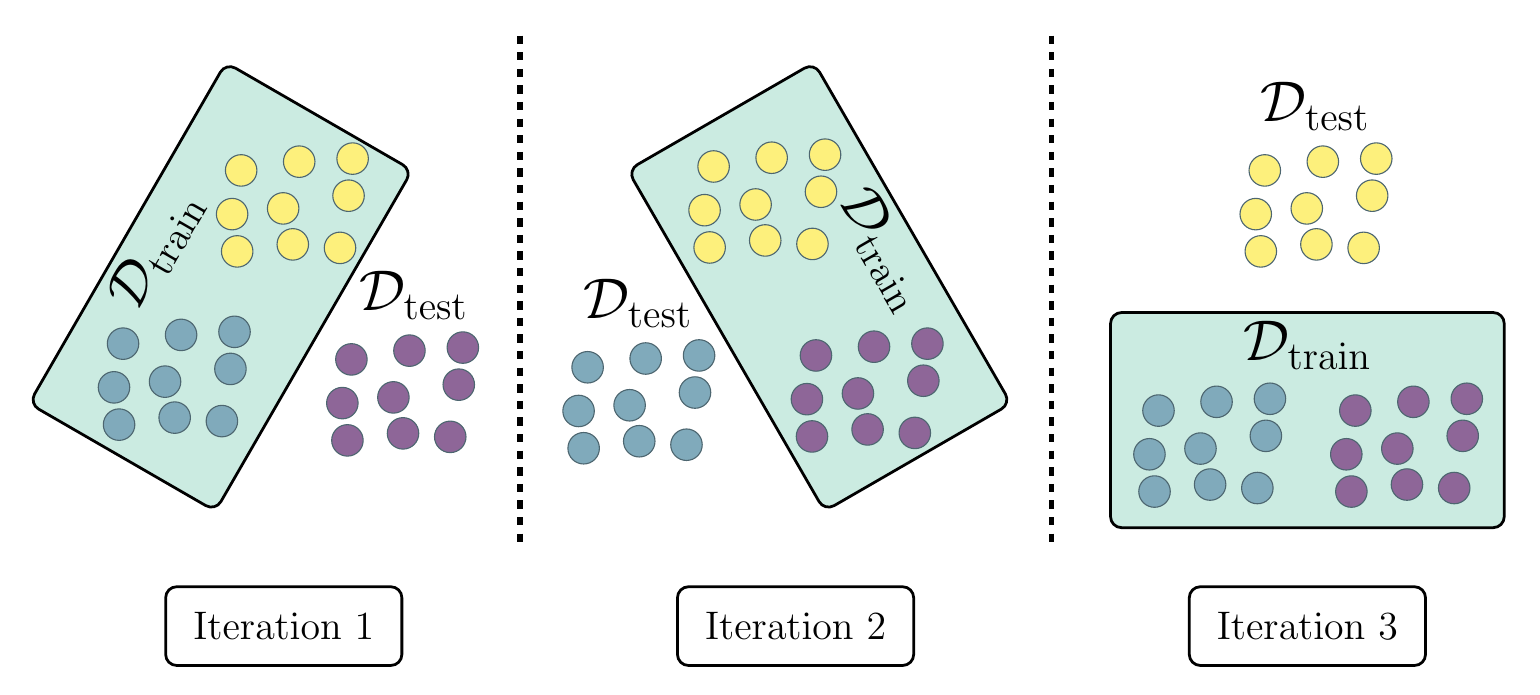
\begin{tikzpicture}[
    scale=1.0,
    every node/.style={
        transform shape,
        minimum width = 50mm,
        minimum height = 20mm,
        fill = viridis6!40,
        rounded corners,
        draw = black,
        line width = 1,
        font = \huge,
        bend angle = 30
    },
    shorten >=0.5pt,
    >={Stealth[round]}
]

% train data
\node[rotate = 60, text depth = 2cm, anchor=north] at (0, 0) {$\Dtrain$};
\node[rotate = -60, text depth = 2cm, anchor=north] at (10, 0) {$\Dtrain$};
\node[text depth = 2cm, anchor=north] at (15, -1) {$\Dtrain$};

% test data
\node[draw = none, fill = none] at (3.65, -0.8) {$\Dtest$};
\node[draw = none, fill = none] at (6.5, -0.9) {$\Dtest$};
\node[draw = none, fill = none] at (15.1, 1.6) {$\Dtest$};

% iterations
\node[fill = white, minimum width = 3cm, minimum height = 1cm, font = \Large] at (2, -5) {Iteration 1};
\node[fill = white, minimum width = 3cm, minimum height = 1cm, font = \Large] at (8.5, -5) {Iteration 2};
\node[fill = white, minimum width = 3cm, minimum height = 1cm, font = \Large] at (15, -5) {Iteration 3};

% lines
\draw[dashed, line width = 2] (5,2.5) -- (5,-4);
\draw[dashed, line width = 2] (11.75,2.5) -- (11.75,-4);

\pgfmathsetseed{1}
\foreach \x in {-0.2, 0.5, 1.2}
\foreach \y in {-1.3, -1.85, -2.4}
{
    \pgfmathrandominteger{\a}{-240}{240}
    \pgfmathrandominteger{\b}{-240}{240}
    \draw[fill = viridis4, draw = viridis4!60!black] (\x + 0.1 + \a*0.0005, \y + 0 + \b*0.0005) circle (0.2);
    \draw[fill = viridis4, draw = viridis4!60!black] (\x + 6 + \a*0.0005, \y - 0.3 + \b*0.0005) circle (0.2);
    \draw[fill = viridis4, draw = viridis4!60!black] (\x + 13.25 + \a*0.0005, \y - 0.85 + \b*0.0005) circle (0.2);
    \draw[fill = viridis9, draw = viridis4!60!black] (\x + 1.6 + \a*0.0005, \y + 2.2 + \b*0.0005) circle (0.2);
    \draw[fill = viridis9, draw = viridis4!60!black] (\x + 7.6 + \a*0.0005, \y + 2.25 + \b*0.0005) circle (0.2);
    \draw[fill = viridis9, draw = viridis4!60!black] (\x + 14.6 + \a*0.0005, \y + 2.2 + \b*0.0005) circle (0.2);
    \draw[fill = viridis1, draw = viridis4!60!black] (\x + 3 + \a*0.0005, \y - 0.2 + \b*0.0005) circle (0.2);
    \draw[fill = viridis1, draw = viridis4!60!black] (\x + 8.9 + \a*0.0005, \y - 0.15 + \b*0.0005) circle (0.2);
    \draw[fill = viridis1, draw = viridis4!60!black] (\x + 15.75 + \a*0.0005, \y - 0.85 + \b*0.0005) circle (0.2);
}

\end{tikzpicture}

\end{document}